\section{How Emotions are Made}
\paragraph{by Lisa Feldman-Barret}

\subsection{Interoception}

Das ständige Gefühl, welches einen \textit{Gefühlszustand} wiedergibt, wird von dem Prozess: \textbf{Interoception}  produziert.\\

\begin{figure}[H]
	\centering
	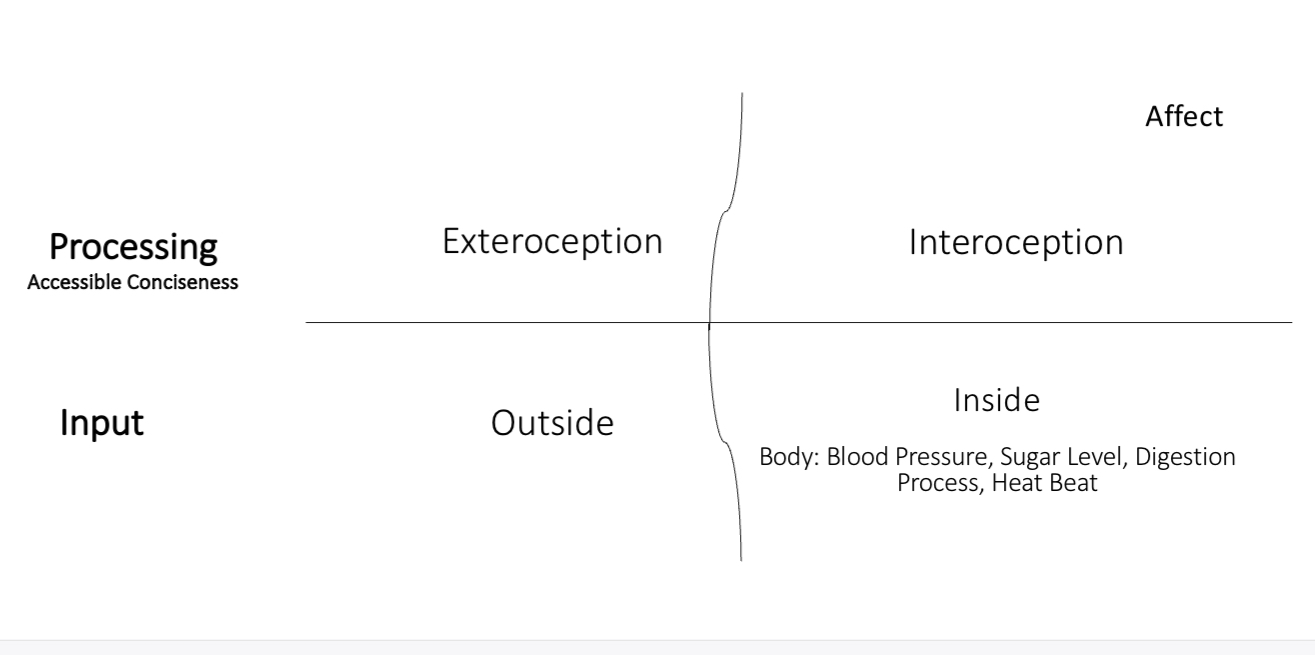
\includegraphics[scale = 0.1]{attachment/chapter_OWN/Scc001}
	\caption{Processing Information}
\end{figure}

The difference between \textit{Interception} and \textit{Extroception} it not as strong as before. The boundry, where you body ends and where the outside world begins is not clear to your brain. It can shift from siutation to situation. eg. driving a car, ganggly teenager. For the feeling of affect outside information can also be used.\\ 

Es geht hier um die Gefühl von Wohlempfinden (Pleasent), Unmut (Unpleasend) und dem Ruhe-Zustand (Calm/ Jitery). Diese Gefühle werden eher als universell gesehen, und heißen \textit{Affect}.  Während Emotionen bieten einen weniger universellen Rahmen.


Interoception, like exteroception, operates in the service of movement predictively. Here’s the gist: Your brain issues motor commands that adjust the insides of your body, and it simultaneously predicts the sensory consequences of those movements. At the same time, the sensory surfaces inside your body, including dozens of cells that monitor pressure changes, temperature, contractions, stretches, nutrients, gases, toxins, and various chemicals, send a steady stream of sensory signals back to your brain via electrical impulses in your spinal cord and swirling chemicals in your blood. Your brain integrates these sensory signals to confirm or correct the predictions and adjust its predicted movements, if necessary, thereby maintaining allostasis efficiently. In this way, your brain anticipates the needs of your body and proactively coordinates the internal movements that deliver glucose, water, salt, oxygen, and other resources to billions of cells just in.\\

%Evolution did not wire us to feel every interoceptive gurgle, gush, and tug directly, so instead, we often experience them as simple feelings: pleasure or displeasure, idleness or activation, fatigue or energy. Scientists call these simple feelings affect or mood. Affect does not reveal what in the world has changed, where the change is, or what to do about it. Rather, it is just a quick and dirty sixth sense that something has happened. That particular something may be outside your body and require a rapid and energetically costly response.

Evolution did not wire us to experience every internal sensation. There are experience as simple feelings, with no directions.\\

%TODO Refactoring

1. Controlled Hallucination: The tool of a  Concept
3. Origin of feeling
2. Emotion are contrustred
4. Concepts, Goals Words


\subsection{Intrinsic Brain Activity}
\subsubsection{Simulation and Prediction}
\subsubsection{Construction Reality}

% TODO: Start
\subsection{Controlled Hallucination}
What our brain does all day, is simulate the world around us. This means, what we precise as reality, is our prediction, what we will percisive as reality. We hallucinate.\\

When we simulate, we are $"$filling$"$ the gaps. The concepts in our head will help us, make sense of the input data, we are receiving. This sense making will also combine information an fill in and ignore information, we are not aware off.

\begin{figure}[H]
	\centering
	\includegraphics[scale = 0.1]{attachment/chapter_OWN/}
	{attachment/chapter_OWN/Scc002}
	\caption{Mystery blobs}
\end{figure}


The two blobs in the figure are to most people just a mystery blos. But if provided with a context, see attachment \textit{How Emotions are made}, the \textbf{Experiential blindness} are overcome, and the figure makes sense. This hallucination is hidden from us. No matter how hard we try, we are not able to oberserve ourself, \underline{constructing} this image or any other image for that matter. Even in this example, we are aware that this process happend, but we cannot experience it. The saying from inception the movie $"$A idea is the most powerfull force in the universe$"$, has some footing, because and idea or a concept is how we shape the universe around as.\footnote{This scientific discovery created a revolution in 1990 in psychology and neuroscience.}\\

